\documentclass[sans]{beamer}

% \usetheme{Boadilla}
\mode<presentation>
{
	% \usetheme{CambridgeUS}
	\usetheme{Hannover}
	% \usetheme{Bergen}
	\usecolortheme{whale}
	% \usefonttheme{serif}
	% \usefonttheme{professionalfonts}
	% \usefonttheme{structureitalicserif}
}

\usepackage{cmap}
\usepackage{listings}
\usepackage{lmodern}
\usepackage{color}
\usepackage{minted}
\usepackage{graphicx}
\usepackage{tikz}
\usepackage{wrapfig}

% \usepackage[labelformat=empty]{subcaption}
\usepackage[labelformat=empty]{caption}

% \usefonttheme{professionalfonts} % using non standard fonts for beamer
% \usefonttheme{sansserif} % default family is serif
% \usepackage{fontspec}
% \usepackage[T2A]{fontenc}
% \setmainfont{Comic Sans MS}

% \usepackage[utf8]{inputenc}
% \usepackage[russian]{babel}

\usepackage{fontspec}
% \setmainfont[Mapping=tex-text]{CMU Serif}



\usepackage{polyglossia}
\setdefaultlanguage{russian}

% \newfontfamily\cyrillicfont[Script=Cyrillic]{Comic Sans MS}
% \newfontfamily{\cyrillicfontt} {Comic Sans MS}
% \newfontfamily{\cyrillicfonttt}{Comic Sans MS}

\setmainfont[Ligatures=TeX]{DejaVu Serif}
\setsansfont[Ligatures=TeX]{DejaVu Sans}
% \setmainfont[Ligatures=TeX]{Comic Sans MS}
% \setsansfont[Ligatures=TeX]{Comic Sans MS}
\setmonofont{DejaVu Sans Mono}

% \setmathfont{XITS Math}
% \defaultfontfeatures{Scale=MatchLowercase,Mapping=tex-text}

\begin{document}

\title[XQuery/XUpdate]{XQuery/XUpdate}

\institute{SE, SPbSU}

\author
[Podkopaev Anton]{Podkopaev Anton, \texttt podkoav239@gmail.com}
\date [07-10-13]{07 October 2013}

\begin{frame}[plain]
	\titlepage
\end{frame}

\section{XQuery}

\begin{frame}{What is XQuery?}
	\begin{columns}
		\begin{column}{0.4\linewidth}
			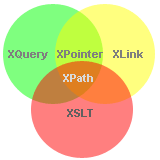
\includegraphics[width = \linewidth]{images/xpath.png}
		\end{column}

		\begin{column}{0.5\linewidth}
			\begin{itemize}
				\item The language for querying XML data
				\item For XML like SQL for databases
				\item Built on XPath expressions
				\item Supported by all major databases
				\item A W3C Recommendation
			\end{itemize}
		\end{column}
	\end{columns}
\end{frame}

\begin{frame}{XQuery and XPath}
	XQuery 1.0 and XPath 2.0 share the same data model and support the same functions and operators

	% Может быть тут написать про XSLT
\end{frame}

% \begin{frame}{Example}
% 	\inputminted{xquery}{codes/ex1.xq}
% \end{frame}

\begin{frame}{Examples of Use}
	\begin{itemize}
		\item Extract information to use in a Web Service
		\item Generate summary reports
		\item Transform XML data to XHTML
		\item Search Web documents for relevant information
	\end{itemize}
\end{frame}

\begin{frame}{XML example}
	\begin{columns}
		\begin{column}{0.45\linewidth}
			\inputminted[fontsize=\tiny]{xml}{codes/ex2.xml}
		\end{column}
		\begin{column}{0.55\linewidth}
			% \begin{block}{Query example}
			\begin{itemize}
				\item \inputminted[fontsize=\tiny]{xquery}{codes/ex3.xq}
				\item \inputminted[fontsize=\tiny]{xquery}{codes/ex4.xq}
			\end{itemize}
			% \end{block}
		\end{column}
	\end{columns}
\end{frame}

\begin{frame}{FLWOR Expressions}
	For, Let, Where, Order by, Return

	\vspace{1cm}

	\begin{block}{Example}
		\inputminted{xquery}{codes/ex5.xq}
	\end{block}
\end{frame}

\begin{frame}{FLWOR + HTML}
	\begin{block}{Script}
		\inputminted[fontsize=\footnotesize]{html}{codes/ex6.html}
	\end{block}

	\begin{block}{Result}
		\inputminted[fontsize=\footnotesize]{html}{codes/ex7.html}
	\end{block}
\end{frame}

\begin{frame}{Custom functions}
	\begin{block}{Syntax}
		\inputminted[fontsize=\tiny]{xquery}{codes/ex8.xq}
	\end{block}
	\begin{block}{Example}
		\inputminted[fontsize=\tiny]{xquery}{codes/ex9.xq}
	\end{block}
\end{frame}

\begin{frame}{Data Types}
	Shares the same data types as XML Schema 1.0 (XSD)

	\begin{itemize}
		\item String
			\begin{itemize}
				\item NormalizedString
				\item Token
				\item ...
			\end{itemize}
		\item Date
		\item Numeric
			\begin{itemize}
				\item Decimal
				\item Integer
				\item ...
			\end{itemize}
		\item Misc
			\begin{itemize}
				\item Boolean
				\item Binary
				\item AnyURI
				\item ...
			\end{itemize}
	\end{itemize}
\end{frame}

\begin{frame}{JSON}
	\begin{itemize}
		\item JSONiq
		\item XQuery 3.1

		\color{blue} \url{w3.org/blog/2013/09/xml-json-xslt-and-xquery/} \color{black}
	\end{itemize}
\end{frame}

% \begin{frame}{Features}
% 	\begin{itemize}
% 		\item Case-sensitive
% 		\item Conditional expressions
% 		\item Custom functions
% 	\end{itemize}
% \end{frame}

\section{XUpdate}

\begin{frame}{What is XUpdate?}
	\begin{itemize}
		\item A lightweight XML query language for modifying XML data
		\item For users not content to wait for the XQuery Update Facility extension of the W3C standard
		\item Last Working Draft, September 14, 2000
	\end{itemize}
\end{frame}

\end{document}